\documentclass[a4paper]{article}
\usepackage{ulem}
\usepackage{graphicx}
\usepackage[namelimits]{amsmath}
\usepackage{amssymb}
\usepackage{amsmath}
\usepackage{amsfonts}
\usepackage{mathrsfs}
\usepackage{enumerate}
\usepackage{indentfirst}
\usepackage{multirow}
\usepackage{latexsym}
\usepackage{subfig}
\usepackage{listings}
\usepackage{xcolor}
\usepackage{algorithm}
\usepackage{algpseudocode}
\usepackage{caption}

\lstset{numbers=left,
	numberstyle=\tiny,
	frame=shadowbox,
	backgroundcolor=\color[RGB]{245,245,244},
	keywordstyle=\color[RGB]{40,40,255},
	numberstyle=\footnotesize\color{darkgray},
	commentstyle=\color[RGB]{50,50,50},
	breaklines=true}

\renewcommand{\algorithmicrequire}{\textbf{Input:}}
\renewcommand{\algorithmicensure}{\textbf{Output:}}

\title{UM-SJTU JOINT INSTITUTE\\VE475 Introduction to Cryptography\\\vspace{0.5cm} Homework 1}
\author{Li Yong 517370910222}
\begin{document}
\maketitle
\newpage

\section*{Ex.1 Simple questions}
	\begin{enumerate}
		\item
		If the key is 4, the plaintext is "ARENA".\\
		If the key is 13, the plaintext is "RIVER".
		\item
		Let the key $K$ be
		$$ K =
		\left(
		\begin{matrix}
			a & b \\
			c & d \\
		\end{matrix}
		\right)
		$$
		Then
		$$
		\underbrace{
		\left(
		\begin{matrix}
			3  & 14 \\
			13 & 19 \\
		\end{matrix}
		\right)}_{A}
		\cdot
		\left(
		\begin{matrix}
			a & b \\
			c & d \\
		\end{matrix}
		\right)
		\equiv
		\left(
		\begin{matrix}
			4  & 11 \\
			13 & 8 \\
		\end{matrix}
		\right)
		\bmod 26
		$$
		$$ K =
		\left(
		\begin{matrix}
			a & b \\
			c & d \\
		\end{matrix}
		\right)
		\equiv
		\left(
		\begin{matrix}
			3  & 14 \\
			13 & 19 \\
		\end{matrix}
		\right)^{-1}
		\cdot
		\left(
		\begin{matrix}
			4  & 11 \\
			13 & 8 \\
		\end{matrix}
		\right)
		\bmod 26
		$$
		$$det(A) = -125 \Rightarrow det(A)\cdot(-5) \equiv 1 \bmod 26
		$$
		So that $A$ is invertible modulo 26 and
		$$A^{-1}=-\frac{1}{125}
		\left(
		\begin{matrix}
			19  & -14 \\
			-13 & 3 \\
		\end{matrix}
		\right) \bmod 26
		$$
		-5 is the inverse of -125 modulo 26, such that
		$$A^{-1}=
		\left(
		\begin{matrix}
			-95 & 70 \\
			65  & -15 \\
		\end{matrix}
		\right)
		\equiv
		\left(
		\begin{matrix}
			9 & 18 \\
			13 & 11 \\
		\end{matrix}
		\right)
		\bmod 26
		$$
		$$K=
		\left(
		\begin{matrix}
			a & b \\
			c & d \\
		\end{matrix}
		\right)
		\equiv
		\left(
		\begin{matrix}
			9 & 18 \\
			13 & 11 \\
		\end{matrix}
		\right)
		\cdot
		\left(
		\begin{matrix}
			4  & 11 \\
			13 & 8 \\
		\end{matrix}
		\right) \bmod 26
		$$
		$$K =
		\left(
		\begin{matrix}
			10  & 9 \\
			13 & 23 \\
		\end{matrix}
		\right)
		$$
	\item
	If $n\mid ab$, then $$ab = cn, c \in \mathbb{Z}.$$
	And gcd$(a, n) = 1$, then there exists two integers $s$ and $t$, such that
	$$as + nt = 1$$
	Multiplying by $b$, we get
	$$asb + ntb = b$$
	$$b = ncs + ntb$$
	$$b = n(cs + tb)$$
	Hence $n|b$.
	\item
	$$
	\begin{aligned}
		30030 &\equiv 218 \bmod 257\\
		257 &\equiv 39 \bmod 218\\
		218 &\equiv 23 \bmod 39\\
		39 &\equiv 16 \bmod 23\\
		23 &\equiv 7 \bmod 16\\
		16 &\equiv 2 \bmod 7\\
		7 &\equiv 1 \bmod 2\\
		2 &\equiv 1 \bmod 1\\
	\end{aligned}
	$$
	Hence gcd$(30030, 257) = 1$.
	$$30030 = 2\times3\times5\times7\times11\times13$$
	These primes are all less than $\sqrt{257}$, hence 257 is prime.
	\item
	Key, plaintext and ciphertext are in the same length. The message with the same key is definitely in the same length. If an attacker knows the key, it will reminds the attacker to use the known key to decrypt the ciphertext. Hence it is dangerous to use the same key twice in the OTP.
	\item
	$$
	\begin{aligned}
		\sqrt{n\log n} &\geq 128\\
		n &\geq 4487
	\end{aligned}
	$$
	\end{enumerate}

\section*{Ex.2 Vigenère cipher}
\begin{enumerate}
	\item The Vigenère cipher encrypts with a table \ref{fig:vigeneretable} (Vigenère square or Vigenère table) which consists of 26 Caesar ciphers in sequence with different shift values. To encrypt, we choose a keyword and repeats it until its length equals to the plaintext's so that we get the key. As for the first letter in the plaintext, we use the Caesar cipher corresponding to the first letter in the key. Then for the second letter of the plaintext, we use the second letter in the key and so on.
	\begin{figure}[!htb]
	\centering
	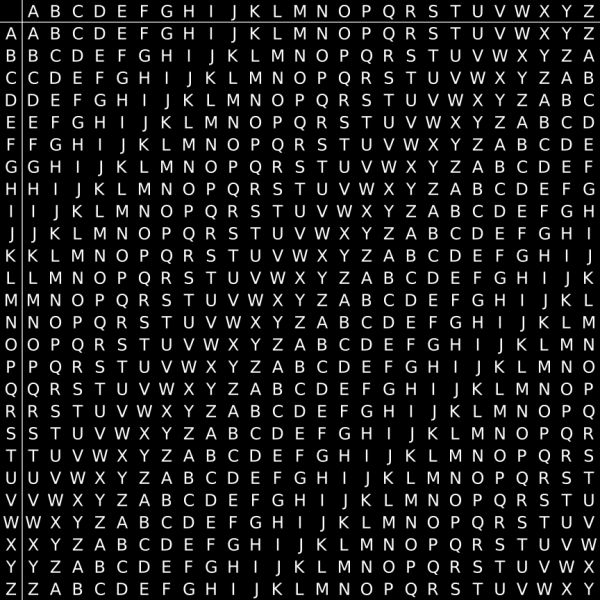
\includegraphics[scale=0.3]{vigeneretable.png}
	\caption{Vigenère square or Vigenère table}
	\label{fig:vigeneretable}
\end{figure}
	\item
	\begin{enumerate}[a)]
		\item Both the plaintext and the key are repeated so that the ciphertext is repeated, the cycle of which is the least common multiple of lengths of the plaintext and the keyword. And the cycle is of 6 letters. Due to repeating so much times, it probably is one repeated letter.
		\item lcd$(1, 6) = 6$, so that Eve can guess the key length is 6.
		\item The ciphertext can also be regarded that the keyword was encrypted by one-letter-key in the Vigenère cipher. Hence, Eve can just decrypt it as a simple Caeser cipher.
	\end{enumerate}
\end{enumerate}

\section*{Ex.3 Programming}
	Uploaded with this PDF.

\end{document}
